\chapter{Benchmark Results}
\label{cha:benchmark}

This chapter reports what the twenty-eight forecasters of Chapter~\ref{cha:baselines}
scored under the protocol of Chapter~\ref{cha:protocol}, and draws four conclusions from
the result. All numbers are cross-plant: fourteen disjoint test plants, fourteen days of
history, a six-hour horizon, capacity-normalised metrics macro-averaged over plants. No
test-plant data entered any fitted component of any model.

\section{Leaderboard}
\label{sec:leaderboard}

\begin{table}[h!]
\centering
\small
\begin{tabular}{r l l c c c c}
\hline
\textbf{\#} & \textbf{Tier} & \textbf{Model} & \textbf{NMAE} $\downarrow$ &
\textbf{NRMSE} $\downarrow$ & \textbf{SS} $\uparrow$ & \textbf{$R^2$} $\uparrow$ \\
\hline
1 & T2 & \textbf{iTransformer} & 0.0699 & 0.1032 & \textbf{0.552} & 0.765 \\
2 & T5 & \textbf{Time-VLM}$^{\dagger}$ & 0.0692 & 0.1061 & \textbf{0.540} & 0.487 \\
3 & T3 & Chronos-2 oracle FT$^{\ddagger}$ & 0.0808 & 0.1142 & 0.504 & 0.706 \\
4 & T4 & TS-RAG & 0.0705 & 0.1203 & 0.478 & 0.331 \\
5 & T4 & Cross-RAG & 0.0726 & 0.1206 & 0.477 & 0.375 \\
6 & T3 & Chronos-2 oracle$^{\ddagger}$ & 0.0817 & 0.1213 & 0.474 & 0.679 \\
7 & T2 & PatchTST & 0.0886 & 0.1249 & 0.458 & 0.651 \\
8 & T6 & Solar-VLM & 0.0955 & 0.1283 & 0.443 & 0.660 \\
9 & T2 & TFT & 0.0889 & 0.1330 & 0.423 & 0.626 \\
10 & T2 & MLP & 0.0958 & 0.1352 & 0.413 & 0.600 \\
11 & T1 & LightGBM & 0.1000 & 0.1419 & 0.384 & 0.555 \\
12 & T4 & CoRA & 0.1025 & 0.1444 & 0.374 & 0.550 \\
13 & T3 & TTM-R2 fine-tuned & 0.1029 & 0.1465 & 0.364 & 0.520 \\
14 & T6 & CrossViVit & 0.1112 & 0.1500 & 0.349 & 0.565 \\
15 & T1 & TabPFN-3 & 0.1076 & 0.1524 & 0.339 & 0.499 \\
16 & T3 & Chronos-2 fine-tuned & 0.1120 & 0.1543 & 0.331 & 0.475 \\
17 & T2 & DLinear & 0.1131 & 0.1556 & 0.325 & 0.462 \\
18 & T3 & TiRex zero-shot & 0.1145 & 0.1642 & 0.287 & 0.440 \\
19 & T3 & TimesFM 2.5 zero-shot & 0.1172 & 0.1680 & 0.271 & 0.429 \\
20 & T0 & Hourly climatology & 0.1353 & 0.1766 & 0.234 & 0.314 \\
21 & T5 & Aurora & 0.1280 & 0.1769 & 0.232 & 0.440 \\
22 & T6 & SUNSET & 0.1384 & 0.1806 & 0.216 & 0.359 \\
23 & T3 & Chronos-2 zero-shot & 0.1376 & 0.1873 & 0.187 & 0.277 \\
24 & T5 & UniCast & 0.1433 & 0.2025 & 0.121 & 0.371 \\
25 & T0 & Seasonal naive & 0.1419 & 0.2058 & 0.107 & 0.276 \\
26 & T5 & VisionTS++ & 0.1690 & 0.2266 & 0.017 & 0.397 \\
27 & T0 & Persistence & 0.1643 & 0.2272 & 0.014 & 0.171 \\
--- & T0 & \emph{Smart persistence} (reference) & 0.1593 & 0.2304 & 0.000 & 0.210 \\
28 & T3 & TTM-R2 zero-shot & 0.1704 & 0.2490 & $-0.081$ & 0.155 \\
\hline
\end{tabular}
\caption{Cross-plant leaderboard on \texttt{uk\_pv} (scenario S2). $^{\dagger}$ non-aligned
evaluation windows, see Section~\ref{sec:implementation}. $^{\ddagger}$ oracle variants
consume observed future weather and are upper bounds, not competitors.}
\label{tab:leaderboard}
\end{table}

\paragraph{Probabilistic scores.} Continuous ranked probability scores are available only
for quantile-native models: Chronos-2 oracle fine-tuned 0.0630, Chronos-2 oracle 0.0635,
TFT 0.0689, LightGBM 0.0768, TabPFN-3 0.0815, CoRA 0.0816, Chronos-2 fine-tuned 0.0855,
Chronos-2 zero-shot 0.1072. The ordering broadly tracks the point metrics with one
instructive exception: TFT ranks ninth on skill but third on calibration. A model can be
mediocre at predicting the conditional mean and excellent at describing its own uncertainty,
and for a grid operator sizing reserve capacity the second property is not a consolation
prize.

\paragraph{Metric disagreement.} NMAE and NRMSE do not induce the same ordering, and the
disagreements are diagnostic. TS-RAG has the second-best NMAE of the whole suite (0.0705)
but only the fourth-best NRMSE, and an $R^2$ of 0.331 --- far below models with similar
skill. It is very accurate on typical steps and poor on the large deviations that squared
error punishes. Solar-VLM shows the opposite profile: a mediocre NMAE with a high $R^2$ of
0.660, meaning it follows the shape of the day closely while being systematically
mis-scaled. The headline skill score, being NRMSE-based, rewards the first pattern less
than a mean-absolute framing would and the second more.

\paragraph{Summary of what follows.} Table~\ref{tab:findings} states the four conclusions
before they are argued, so that a reader can check each against the leaderboard directly.

\begin{table}[h!]
\centering
\small
\begin{tabular}{p{5.4cm} p{8.0cm}}
\hline
\textbf{Finding} & \textbf{Evidence} \\
\hline
A well-tuned supervised transformer is the model to beat &
iTransformer 0.552, ahead of every foundation model, retrieval scheme and multimodal system \\
Zero-shot foundation models underdeliver &
0.187, 0.271, 0.287 and $-0.081$ across three architecture families; three of four below
climatology \\
Retrieval beats fine-tuning on a frozen backbone &
0.478 against 0.331 for the same backbone, with no weight update \\
Genuine exogenous imagery has not paid off &
Best multimodal model (0.540) uses rendered images; every satellite-consuming model ranks
eighth or below \\
\hline
\end{tabular}
\caption{The four findings and the evidence for each, stated in advance of the argument.}
\label{tab:findings}
\end{table}

\section{Reading by tier}
\label{sec:by-tier}

\paragraph{Tier 0.} The reference tier spans a wide range, which is itself informative.
Hourly climatology reaches 0.234 --- a model with no knowledge of the current day beats
naive persistence (0.014) by a wide margin, and beats three of the four zero-shot foundation
models. The gap between persistence and smart persistence is instructive in the other
direction: they score 0.014 and 0.000 on skill respectively, yet smart persistence is the
harder reference in every regime that matters, because the skill score is defined relative
to it and persistence's apparent edge comes from the trivially predictable diurnal
component.

\paragraph{Tiers 1 and 2.} Supervised models dominate the upper half of the table.
iTransformer leads outright; PatchTST is seventh; TFT, MLP and LightGBM occupy ninth
through eleventh. DLinear at 0.325 is the informative low end: a single linear layer on a
trend/seasonal decomposition, consuming no covariates, essentially matches fine-tuned
Chronos-2 (0.331). Whatever the pretrained model contributes on this task, it is worth
approximately as much as a linear layer with the right decomposition.

\paragraph{Tier 3.} The foundation-model tier is bimodal. Zero-shot rows occupy positions
18, 19, 23 and 28; adapted rows occupy 13 and 16; oracle rows sit at 3 and 6. The spread
within a single backbone --- Chronos-2 ranges from 0.187 zero-shot to 0.504 with oracle
covariates --- is larger than the spread across the entire supervised tier. On this task,
what a foundation model is \emph{conditioned on} matters more than which foundation model it
is.

\paragraph{Tier 4.} The two retrieval methods are nearly tied at 0.478 and 0.477 and are the
best non-oracle results built on a foundation model. CoRA trails at 0.374. The ordering
within the tier is the interesting part and is developed in Section~\ref{sec:finding3}.

\paragraph{Tiers 5 and 6.} The multimodal tiers straddle the whole table. Time-VLM is second
overall; every other multimodal model is eighth or below, and four of the seven fall in the
bottom third. The split does not follow tier boundaries --- it follows the
endogenous/exogenous boundary, which is the subject of Section~\ref{sec:finding4}.

\section{Tier-level summary}
\label{sec:tier-summary}

Table~\ref{tab:tier-summary} aggregates the leaderboard by tier. With four to eight models per
tier these are small samples and the spread matters more than the mean, but the pattern is
stable enough to be worth stating.

\begin{table}[h!]
\centering
\small
\begin{tabular}{l c c c c}
\hline
\textbf{Tier} & \textbf{Models} & \textbf{Best SS} & \textbf{Median SS} & \textbf{Worst SS} \\
\hline
T0 Reference & 4 & 0.234 & 0.061 & 0.000 \\
T1 Classical ML & 2 & 0.384 & 0.362 & 0.339 \\
T2 Supervised DL & 5 & \textbf{0.552} & 0.423 & 0.325 \\
T3 Foundation (honest) & 6 & 0.364 & 0.301 & $-0.081$ \\
T3 Foundation (oracle) & 2 & 0.504 & 0.489 & 0.474 \\
T4 Frozen adaptation & 3 & 0.478 & 0.477 & 0.374 \\
T5 Endogenous multimodal & 4 & 0.540 & 0.177 & 0.017 \\
T6 Exogenous multimodal & 3 & 0.443 & 0.349 & 0.216 \\
\hline
\end{tabular}
\caption{Leaderboard aggregated by tier. Median is over the models within the tier. Oracle
rows are separated from the honest foundation-model rows because they are upper bounds.}
\label{tab:tier-summary}
\end{table}

Three readings. The supervised tier has both the best model and a high median, so its strength
is not one lucky architecture. The honest foundation-model tier has the worst median of any
learned tier and by far the widest spread, which is the bimodality of
Section~\ref{sec:by-tier} showing up as a statistic. And the two multimodal tiers differ in a
revealing way: the endogenous tier has the higher ceiling (0.540 against 0.443) and the lower
median (0.177 against 0.349), meaning it contains both the best multimodal model and most of
the worst ones. Rendering a series as an image is a high-variance strategy; consuming
satellite frames is a consistently mediocre one.

\section{Finding 1: a well-tuned supervised transformer is the model to beat}
\label{sec:finding1}

iTransformer tops every metric --- skill 0.552, $R^2$ 0.765, best NRMSE --- ahead of every
foundation model, every retrieval scheme and every multimodal system in the suite. The lead
is not marginal: 0.074 skill clear of the best non-oracle foundation-model result and 0.221
clear of honest Chronos-2 fine-tuning.

This inverts the usual framing and deserves to be stated without softening. On this task,
architecture plus in-domain supervised training on 69 plants beats large-scale pretraining.
The comparison is fair in the strongest sense: the supervised models also see only training
plants, are also evaluated on disjoint test plants, and receive the same windows and the same
covariates. They have no pretraining and no privileged information.

Why iTransformer specifically? Its inductive bias matches the structure of the problem
unusually well. It applies attention across \emph{variates} rather than across time, treating
each channel as a token, and Figure~\ref{fig:correlations} shows why that pays: normalised
power correlates at 0.74 with shortwave radiation, 0.69 with direct radiation and 0.60 with
direct normal irradiance, while the covariates are heavily correlated with each other
(0.93 between shortwave and direct radiation). The forecasting problem is substantially a
problem of resolving a small set of strongly inter-correlated exogenous drivers, and
variate-attention models exactly that. PatchTST, which is channel-independent, ranks seventh;
the difference between the two is a clean demonstration that on this task the cross-channel
structure is where the signal is.

The finding does not show that pretraining is worthless. It shows that on a task with 69
training plants and a strongly structured covariate track, the value of pretraining is
smaller than the value of a well-matched inductive bias --- and that a paper reporting only
foundation-model comparisons would have reached the opposite conclusion by omission.

\section{Finding 2: zero-shot foundation models underdeliver}
\label{sec:finding2}

The zero-shot tier is the weakest part of the leaderboard. Chronos-2 scores 0.187, TimesFM
0.271, TiRex 0.287, and TTM-R2 reaches $-0.081$ --- worse than assuming cloud conditions
persist. All four trail LightGBM; three of the four trail hourly climatology, a model that
has never seen the current day.

Because the result replicates across an encoder transformer, a decoder transformer and a
mixer architecture, it is a property of the task rather than of any one pretraining corpus.
The natural explanation is distributional. Photovoltaic power is bounded below by zero and
above by capacity, is gated by a deterministic astronomical cycle, is exactly zero for a
large and predictable fraction of every day, and transitions abruptly when a cloud edge
crosses the array (Figure~\ref{fig:ramps}). General-purpose pretraining corpora are dominated
by smooth economic, demand and sensor series with none of those properties. A model whose
prior is ``series are smooth and roughly stationary in the short run'' is systematically
wrong here in a way that no amount of context length repairs.

Two secondary observations support the reading. First, the failure is worst for the smallest
model: TTM-R2 zero-shot is the only entry below the reference floor, and fine-tuning the same
architecture recovers it to 0.364 --- a swing of 0.445 skill from adaptation alone. The
zero-shot deficit is therefore not a capacity ceiling but a prior mismatch. Second, the
ordering among zero-shot models does not track their general-purpose leaderboard ordering,
which is what one expects if the limiting factor is domain mismatch rather than model
quality.

Adaptation is not optional on this task. That conclusion is what makes Tier~4 the interesting
tier rather than a completeness exercise.

\section{Finding 3: retrieval beats fine-tuning on a frozen backbone}
\label{sec:finding3}

Every adaptation step helps --- Chronos-2 moves from 0.187 to 0.331, TTM-R2 from $-0.081$ to
0.364 --- but the ordering \emph{among} adaptation strategies is the result worth carrying
forward. Retrieval over a frozen backbone reaches 0.478 (TS-RAG) and 0.477 (Cross-RAG)
against 0.331 for fine-tuning the same backbone: 0.147 skill, obtained without a single
gradient update to the model.

The covariate adapter sits between them at 0.374, which sharpens the interpretation. What
retrieval supplies is not simply ``more input'' --- CoRA also supplies more input, in the form
of the full covariate track, and gains less. What retrieval supplies is \emph{relevant
precedent}: windows whose dynamics resemble the current one. For a problem whose central
difficulty is regime identification --- is this a clear day, a broken-cloud day, or a front
passing? --- an example of how a similar situation evolved is worth more than either a
re-fitted weight matrix or an additional covariate channel.

There is a caveat that keeps this from being a stronger claim than it is. The two retrieval
models have low $R^2$ (0.331 and 0.375) relative to their skill, and Section~\ref{sec:leaderboard}
noted the same pattern in their metric disagreement. They are excellent on typical steps and
comparatively weak at tracking the day's shape, which suggests they are exploiting the
datastore for level calibration at least as much as for dynamics. Whether the gain would
survive a harder ramp-weighted evaluation is visible in Appendix~\ref{app:ramp}, where both
sit mid-table on ramp NRMSE despite their aggregate rank.

\section{Finding 4: genuine exogenous imagery has not paid off}
\label{sec:finding4}

The best multimodal model in the suite is Time-VLM at 0.540 --- second overall,
statistically level with iTransformer, and with the lowest ramp NRMSE of the entire suite
(0.172, Appendix~\ref{app:ramp}), which is precisely where a visual model is supposed to win.
And Time-VLM consumes \emph{no external imagery at all}: it renders the numerical series as
an image and passes it to pretrained vision-language backbones.

Every model that ingests real satellite frames ranks eighth or below: Solar-VLM 0.443,
CrossViVit 0.349, SUNSET 0.216, UniCast 0.121. The domain state of the art, with genuine
satellite input and a vision-language backbone, trails a model that only ever saw a plot of
its own input by 0.097 skill.

Three explanations are available, and they have very different consequences for the design of
a multimodal forecaster.

\begin{enumerate}
  \item \textbf{Redundancy.} The information in a satellite crop is already present in the
    covariate track. Cloud cover, shortwave radiation and direct normal irradiance are
    supplied numerically to every Tier-2 and Tier-4 model, so the frames may add nothing that
    the reanalysis has not already summarised.
  \item \textbf{Interface loss.} The information is present in the frames but does not survive
    the encoder-to-forecaster interface. A visual encoder trained on natural video produces
    representations optimised for object and motion semantics, not for the quantity a
    forecaster needs, and the learned adapter may be too weak a bridge.
  \item \textbf{Inductive bias, not information.} What converts into skill in Time-VLM is the
    \emph{prior structure} of a visual backbone applied to data the model already had --- and
    that resource is available without any external sensor.
\end{enumerate}

Figure~\ref{fig:cloud-residual} is evidence against the first explanation, and it is worth
dwelling on. It bins daytime observations by shortwave radiation and, within each bin, by
cloud cover. If the reanalysis irradiance already captured everything, the three cloud-cover
boxes within an irradiance bin would coincide. They do not: in the 250--450\,W/m$^2$ bin the
median normalised power falls from 0.33 under clear skies to 0.27 under mixed conditions to
0.24 under overcast, a monotone residual effect that persists across every irradiance bin.
There is genuine cloud-state information beyond what the numerical irradiance channel carries.
That is exactly the information a satellite frame observes directly, and exactly the
information the exogenous models are failing to convert.

The remaining explanations are therefore the second and third, and they are distinguishable
only by controlled experiment --- specifically by the shuffled-frames and modality-grid
controls specified in Chapter~\ref{cha:expdesign}. This is the central open question the
benchmark leaves behind, and it reframes the thesis: the interesting question is no longer
``does deep fusion beat late fusion'' but ``does any current visual interface transmit what
the frames contain''.

\section{Qualitative behaviour}
\label{sec:qualitative}

Aggregate metrics hide failure modes that a plot exposes immediately. Figure~\ref{fig:traces}
shows one forecast window on a representative test plant; Figure~\ref{fig:scatter} contrasts
four models' calibration pooled over all of that plant's windows.

\begin{figure}[h!]
\centering
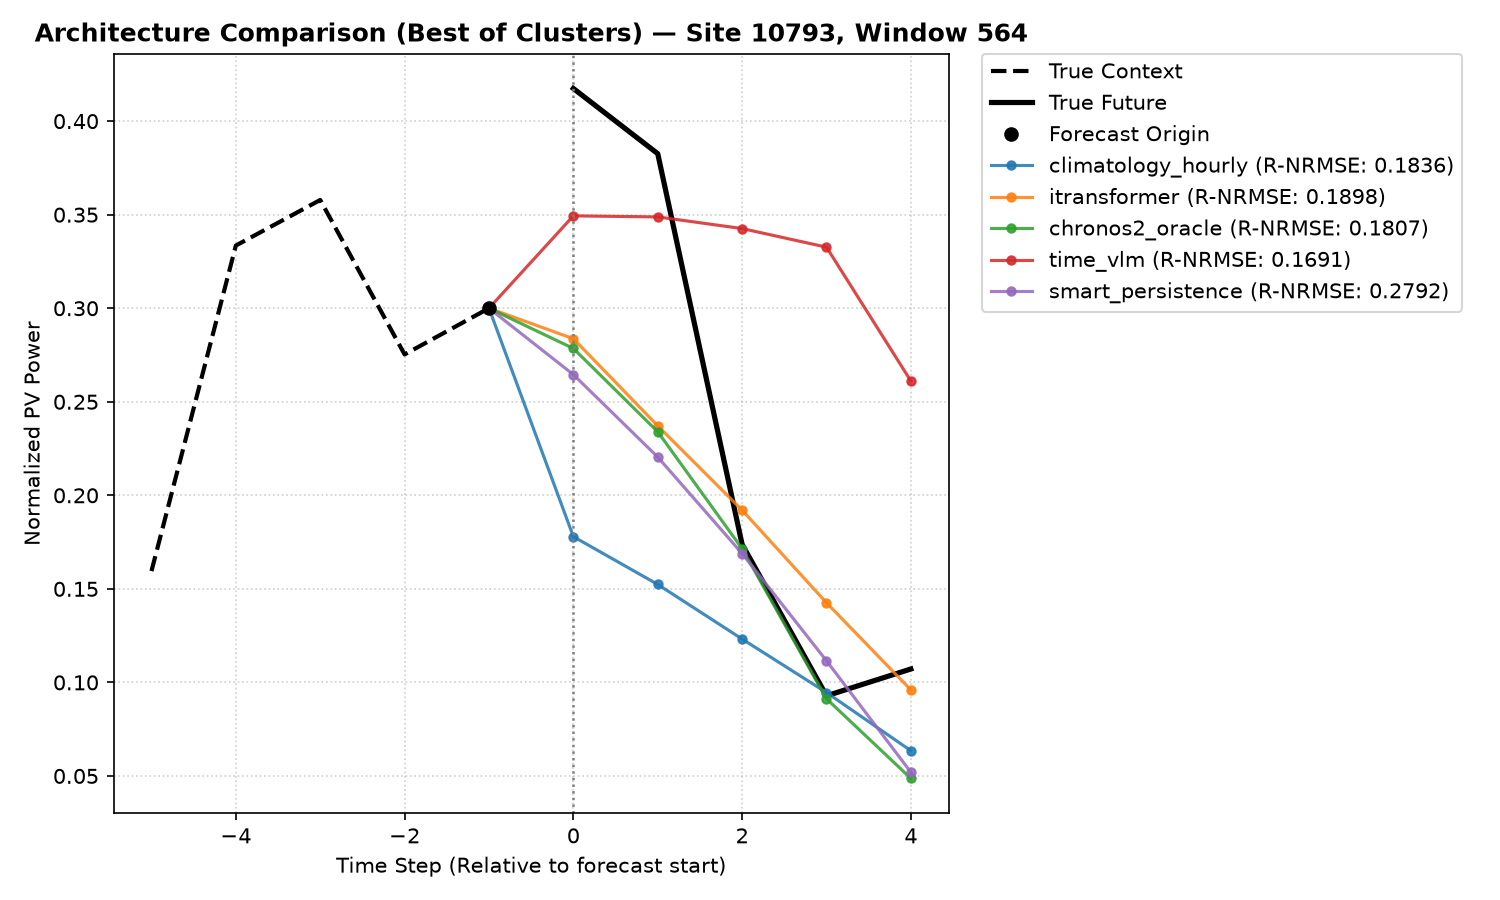
\includegraphics[width=0.92\textwidth]{figures/traces_comparison.png}
\caption{One forecast window on test site 10793: the best model of each cluster against the
truth. Time-VLM is the only model that anticipates elevated output at the start of the
horizon; the others decay smoothly from the forecast origin in the manner of persistence,
and all of them miss the sharp drop at step~2. Legend metrics are window-local and are not
the pooled numbers of Table~\ref{tab:leaderboard}.}
\label{fig:traces}
\end{figure}

The trace exhibits the characteristic failure of the whole suite. The truth rises above the
forecast origin, holds, then falls by three quarters within two steps. Every model except
Time-VLM produces a monotone decay from the origin --- the shape a model outputs when it has
no information about what is about to happen and falls back on the conditional mean. Even
Time-VLM, which correctly holds output high for two steps, misses the drop entirely and ends
the horizon far above the truth. The models are not disagreeing about the ramp; they are
collectively blind to it.

\begin{figure}[h!]
\centering
\begin{minipage}{0.48\textwidth}
  \centering
  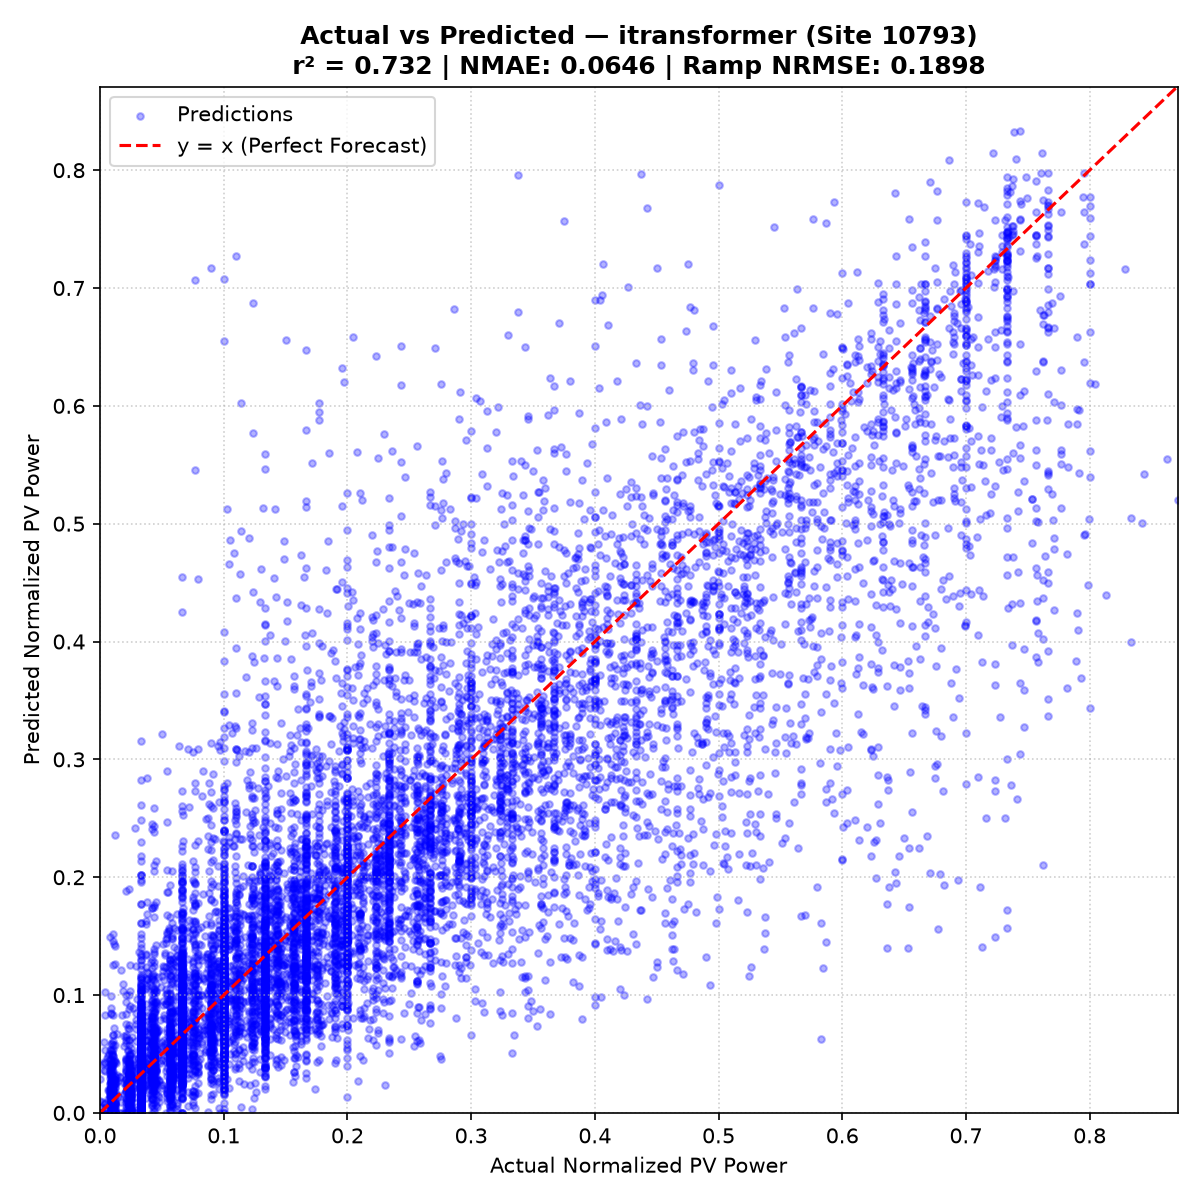
\includegraphics[width=\textwidth]{figures/scatter_itransformer.png}
\end{minipage}
\hfill
\begin{minipage}{0.48\textwidth}
  \centering
  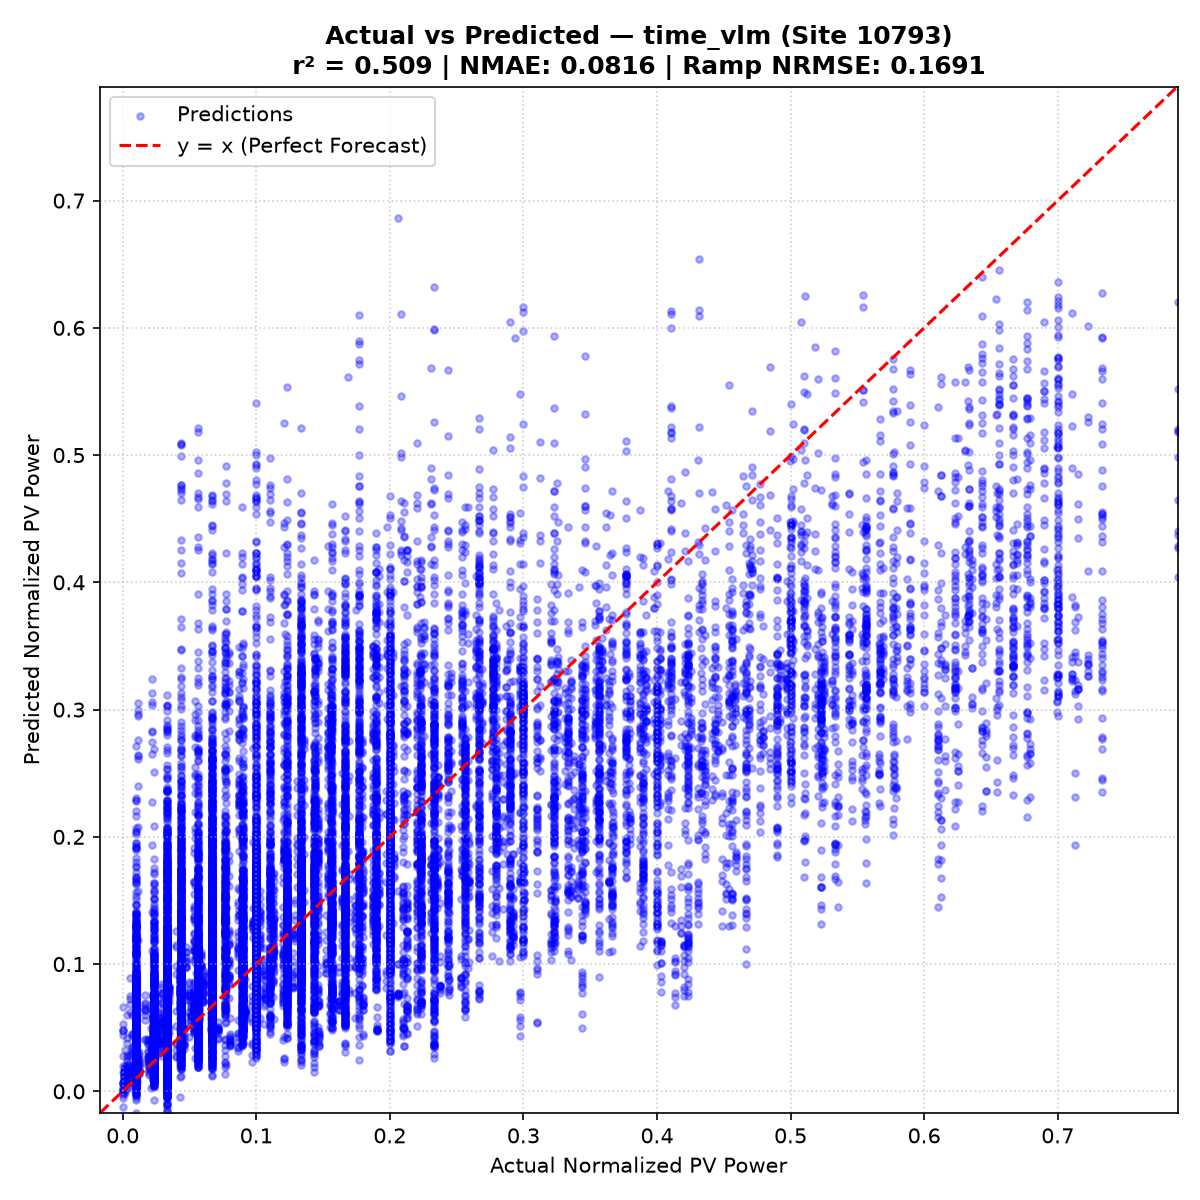
\includegraphics[width=\textwidth]{figures/scatter_time_vlm.png}
\end{minipage}

\vspace{0.35cm}

\begin{minipage}{0.48\textwidth}
  \centering
  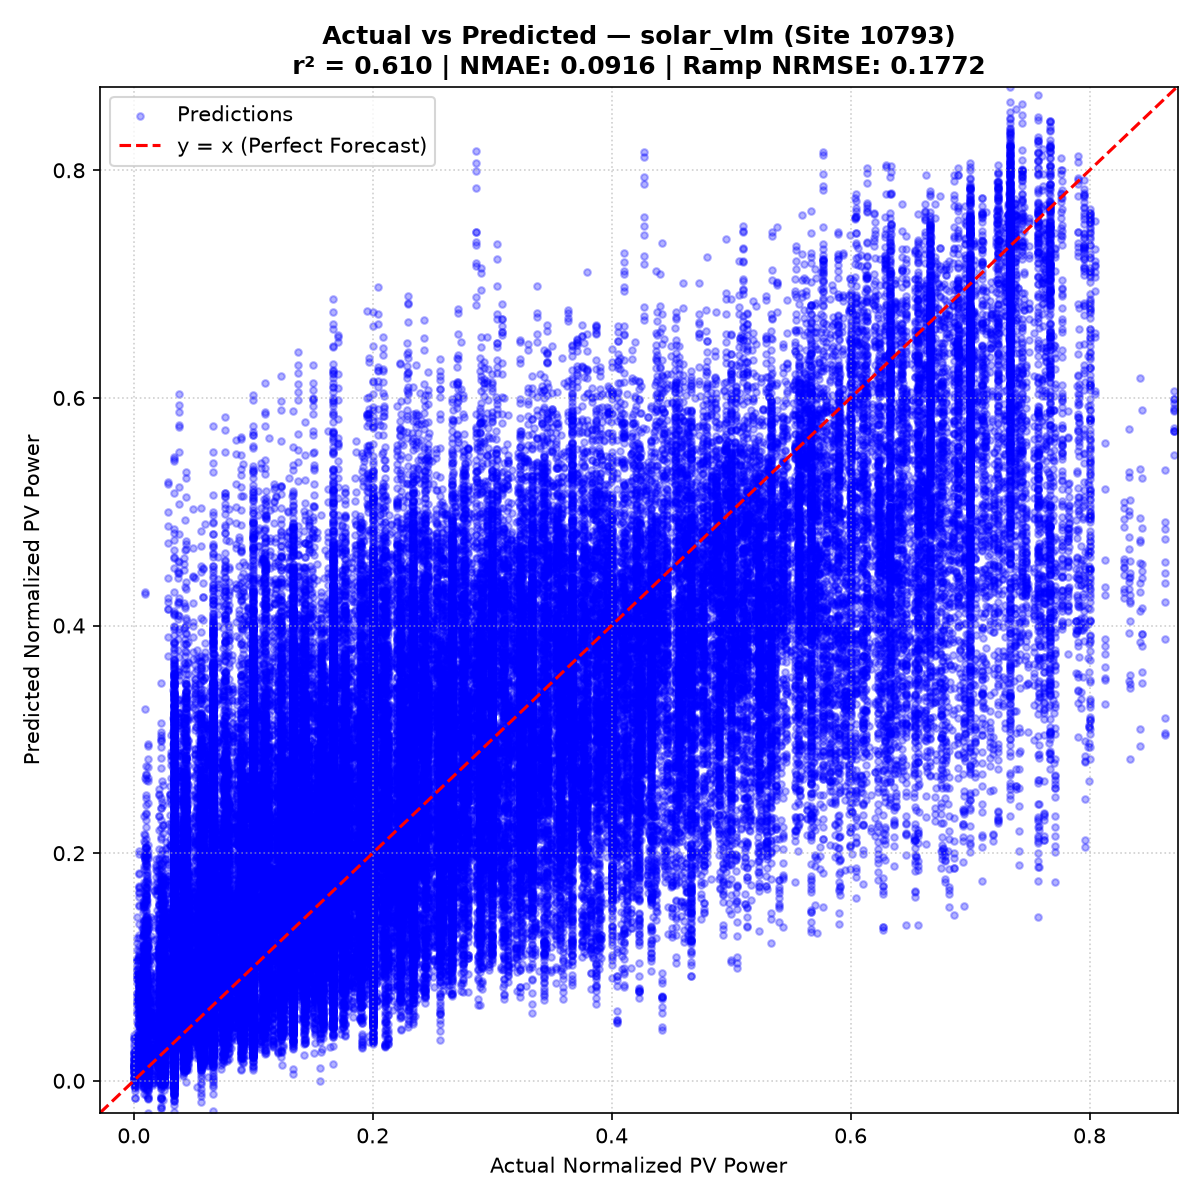
\includegraphics[width=\textwidth]{figures/scatter_solar_vlm.png}
\end{minipage}
\hfill
\begin{minipage}{0.48\textwidth}
  \centering
  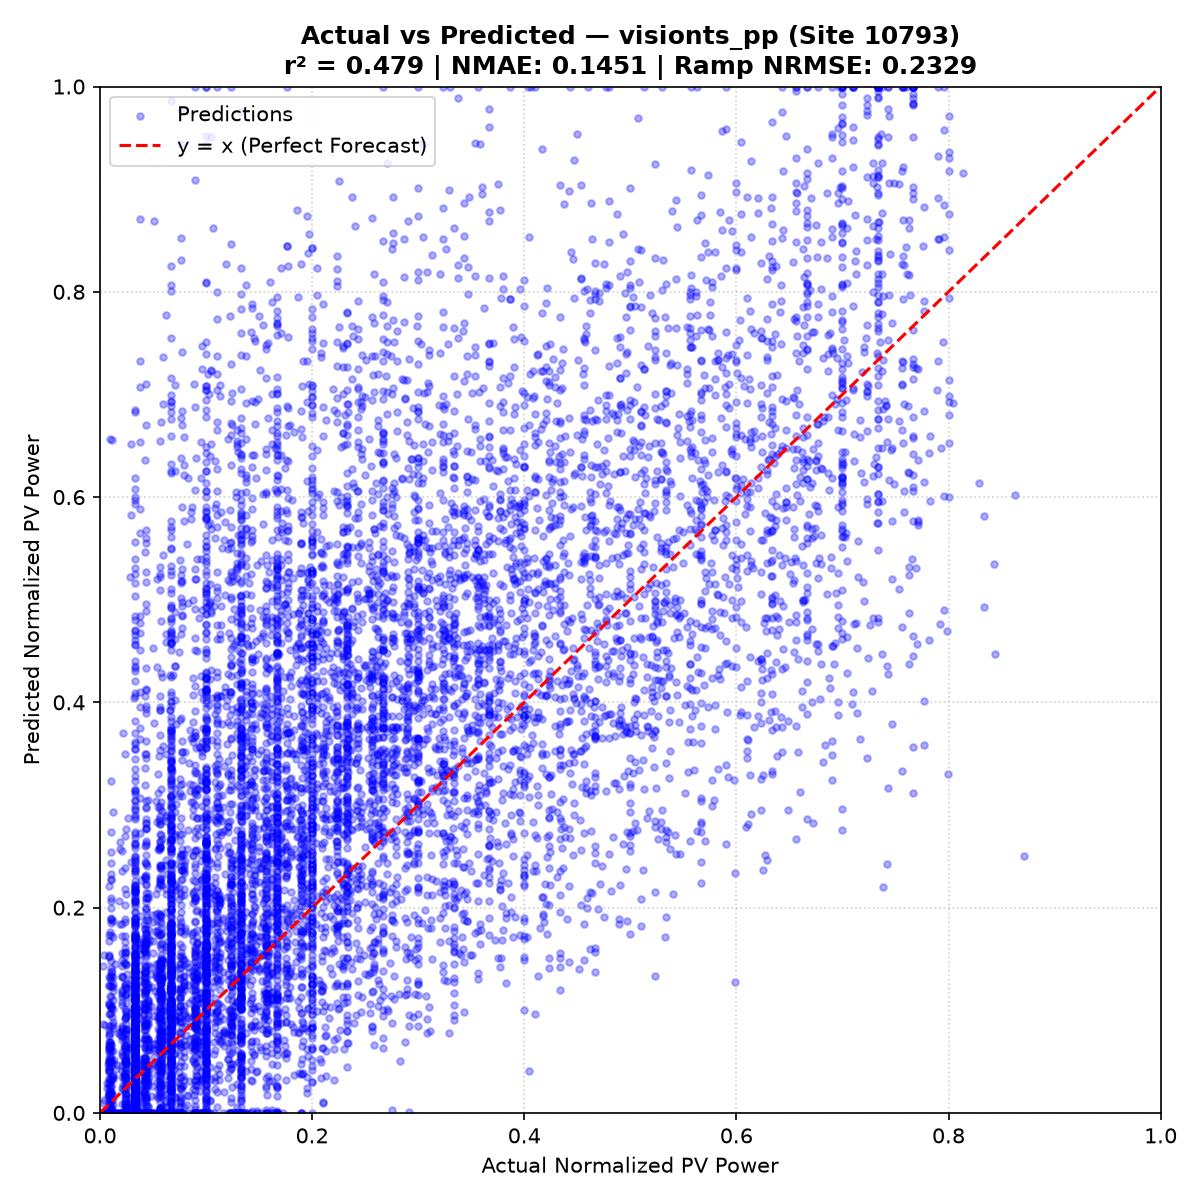
\includegraphics[width=\textwidth]{figures/scatter_visionts_pp.png}
\end{minipage}
\caption{Actual against predicted power on test site 10793, pooled over all windows. Top:
iTransformer and Time-VLM, the two leaders, both tightly distributed about the diagonal.
Bottom: Solar-VLM, which tracks shape but sits below the diagonal at high output, and
VisionTS++, whose cloud is over-dispersed and biased upward at low power. Per-panel metrics
are site-local and are \emph{not} the pooled fourteen-plant numbers of
Table~\ref{tab:leaderboard}.}
\label{fig:scatter}
\end{figure}

Two distinct pathologies appear in the scatter plots, and neither is visible in a skill
column. Several exogenous multimodal models --- Solar-VLM, SUNSET, CrossViVit ---
\emph{systematically under-predict}: they track the shape of the day well ($R^2$ between 0.36
and 0.66) yet sit below the diagonal at high output. VisionTS++ fails differently, with an
over-dispersed cloud biased upward at low power: respectable variance tracking ($R^2$ 0.397)
and almost no skill (0.017), because it is wrong about magnitude in both directions rather
than consistently in one. UniCast is the cleanest instance of the first pathology, with
predictions of approximately $0.61\,y + 0.063$ at correlation 0.61, compounded by a late-day
skew in its native evaluation windows.

\begin{figure}[h!]
\centering
\begin{minipage}{0.48\textwidth}
  \centering
  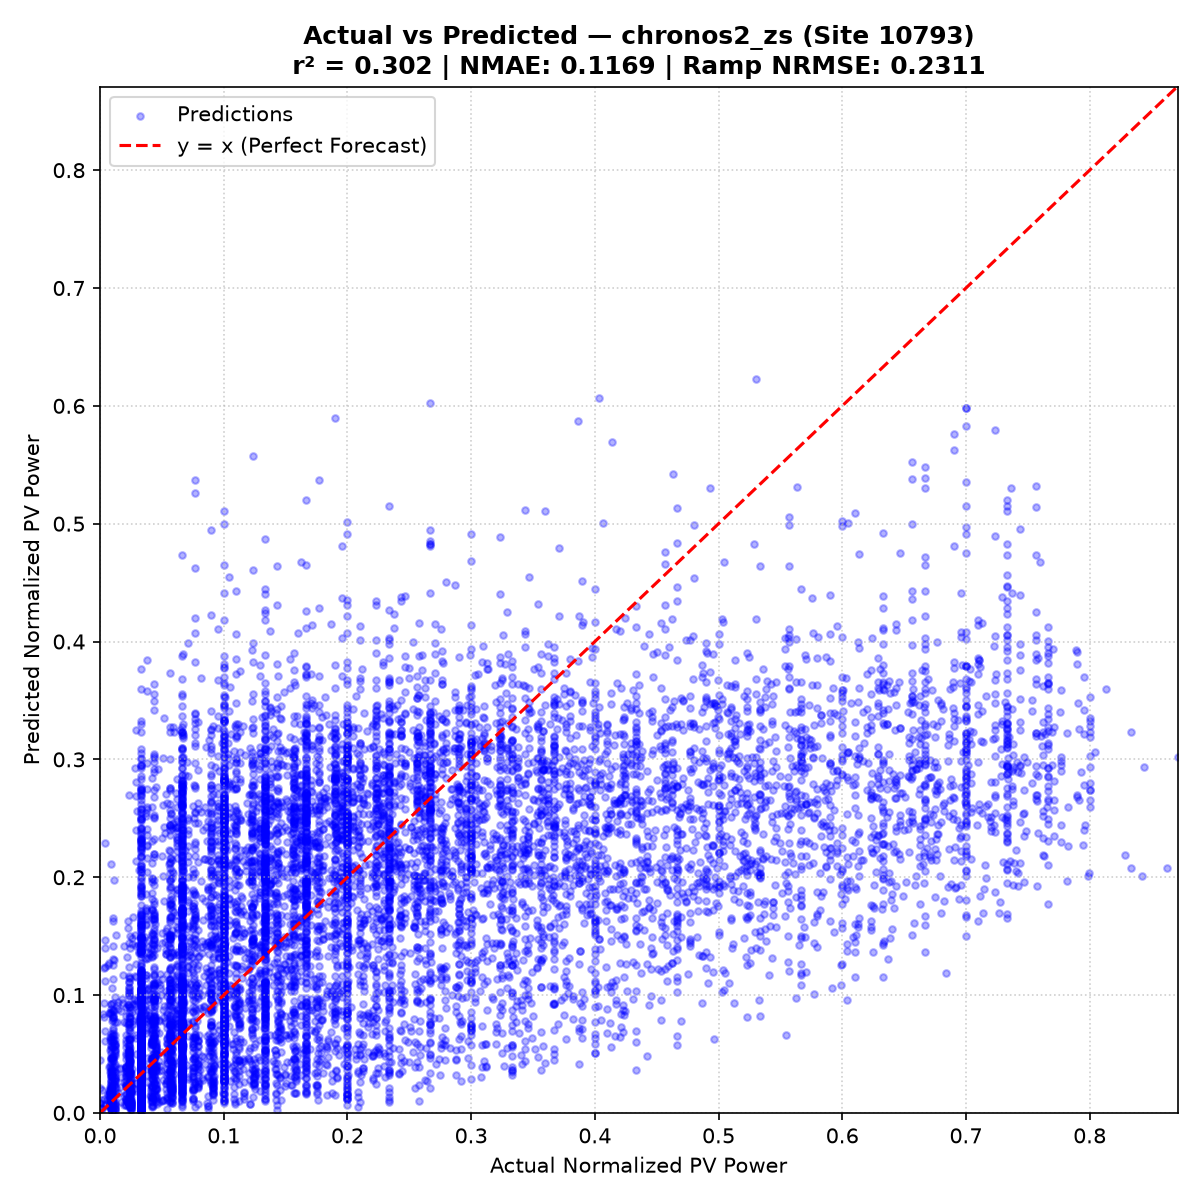
\includegraphics[width=\textwidth]{figures/scatter_chronos2_zs.png}
\end{minipage}
\hfill
\begin{minipage}{0.48\textwidth}
  \centering
  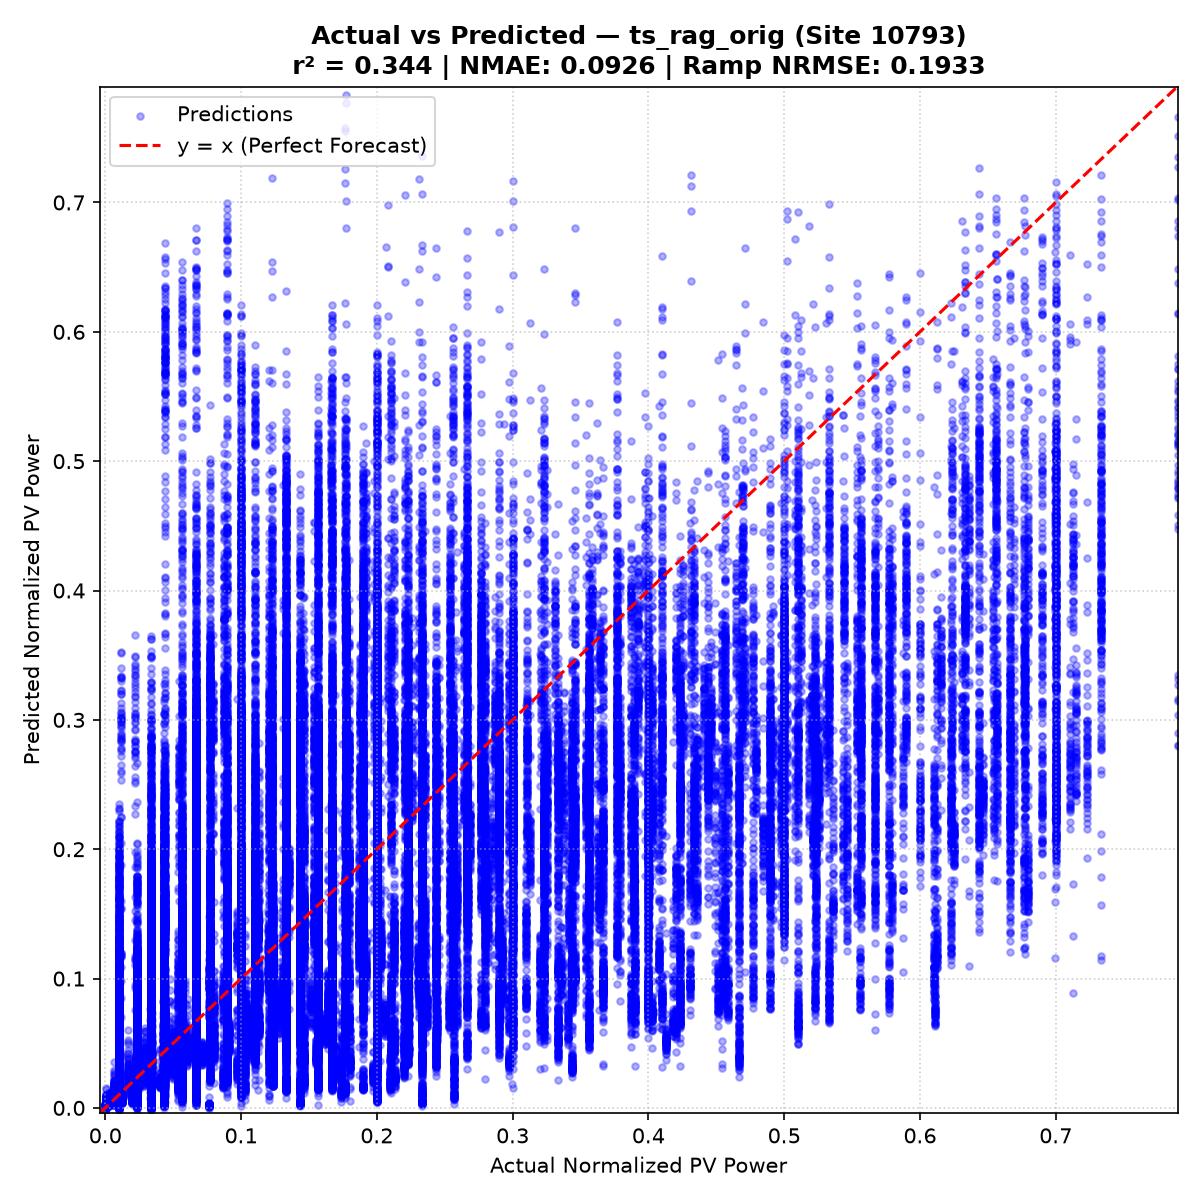
\includegraphics[width=\textwidth]{figures/scatter_ts_rag_orig.png}
\end{minipage}
\caption{The effect of retrieval on a frozen backbone, same test site. Left: Chronos-2
zero-shot. Right: TS-RAG over the same frozen backbone. Retrieval tightens the distribution
substantially without any weight update.}
\label{fig:scatter-rag}
\end{figure}

Both pathologies are \emph{bias and scale} failures rather than timing failures, and both are
in principle recoverable by recalibration. Recalibration was not attempted, for two reasons.
It would have to be fitted on validation plants only, to avoid the leakage the protocol
forbids; and more fundamentally it would change what the tier measures, converting a
comparison of forecasters into a comparison of forecasters-plus-post-processing. The honest
reading is that several published multimodal architectures transfer their \emph{shape}
knowledge across plants but not their \emph{scale} knowledge --- which is itself a finding
about cross-plant generalisation, and one that capacity normalisation was supposed to prevent.

\begin{figure}[h!]
\centering
\begin{minipage}{0.48\textwidth}
  \centering
  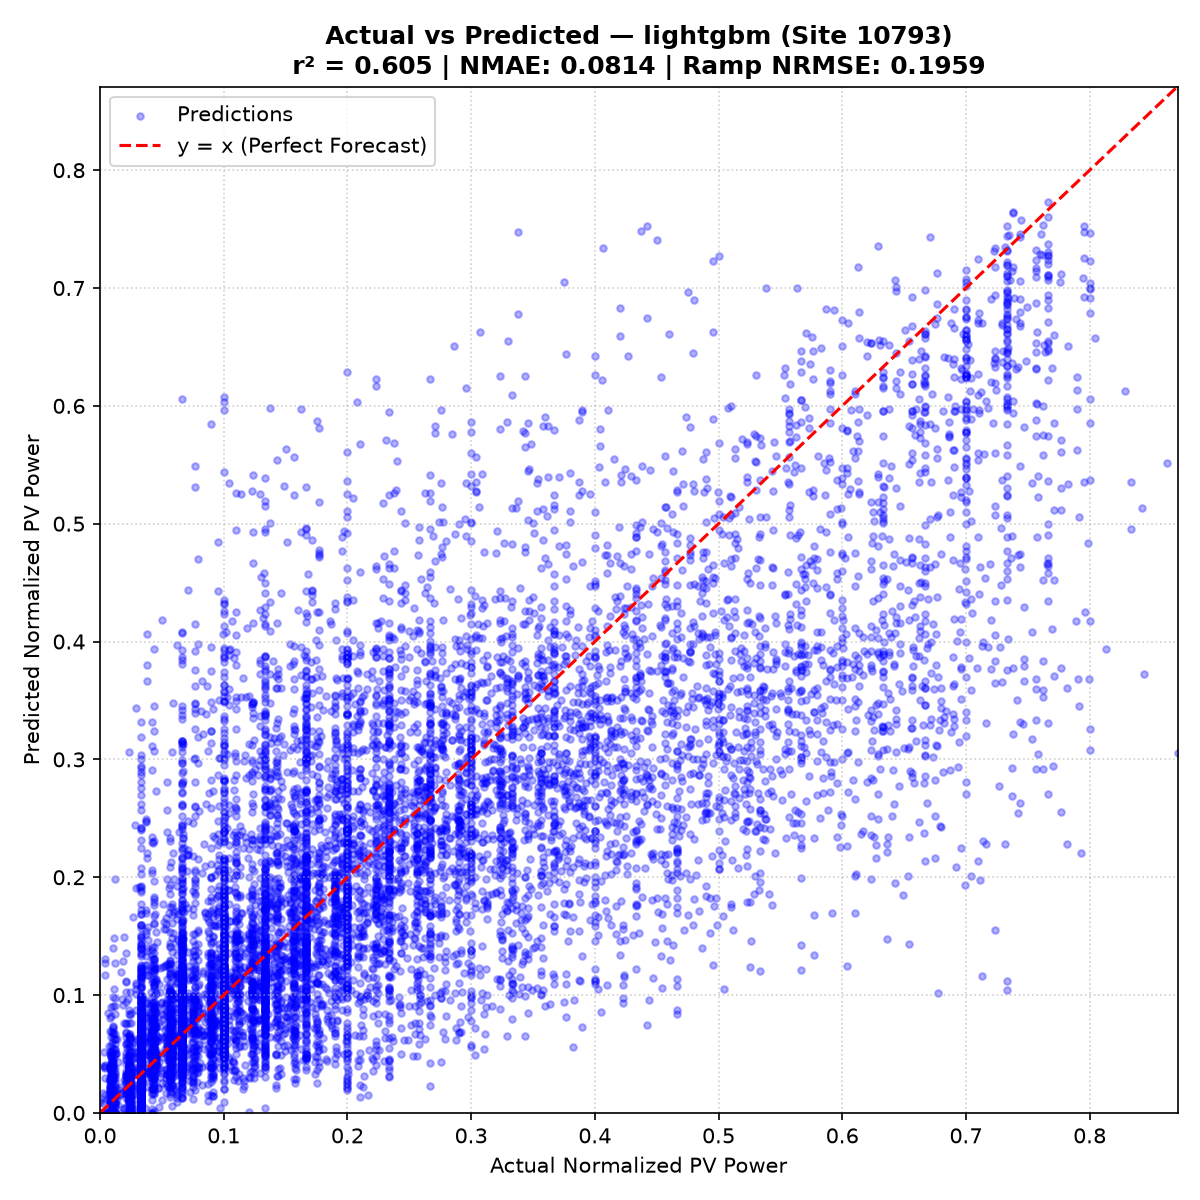
\includegraphics[width=\textwidth]{figures/scatter_lightgbm.png}
\end{minipage}
\hfill
\begin{minipage}{0.48\textwidth}
  \centering
  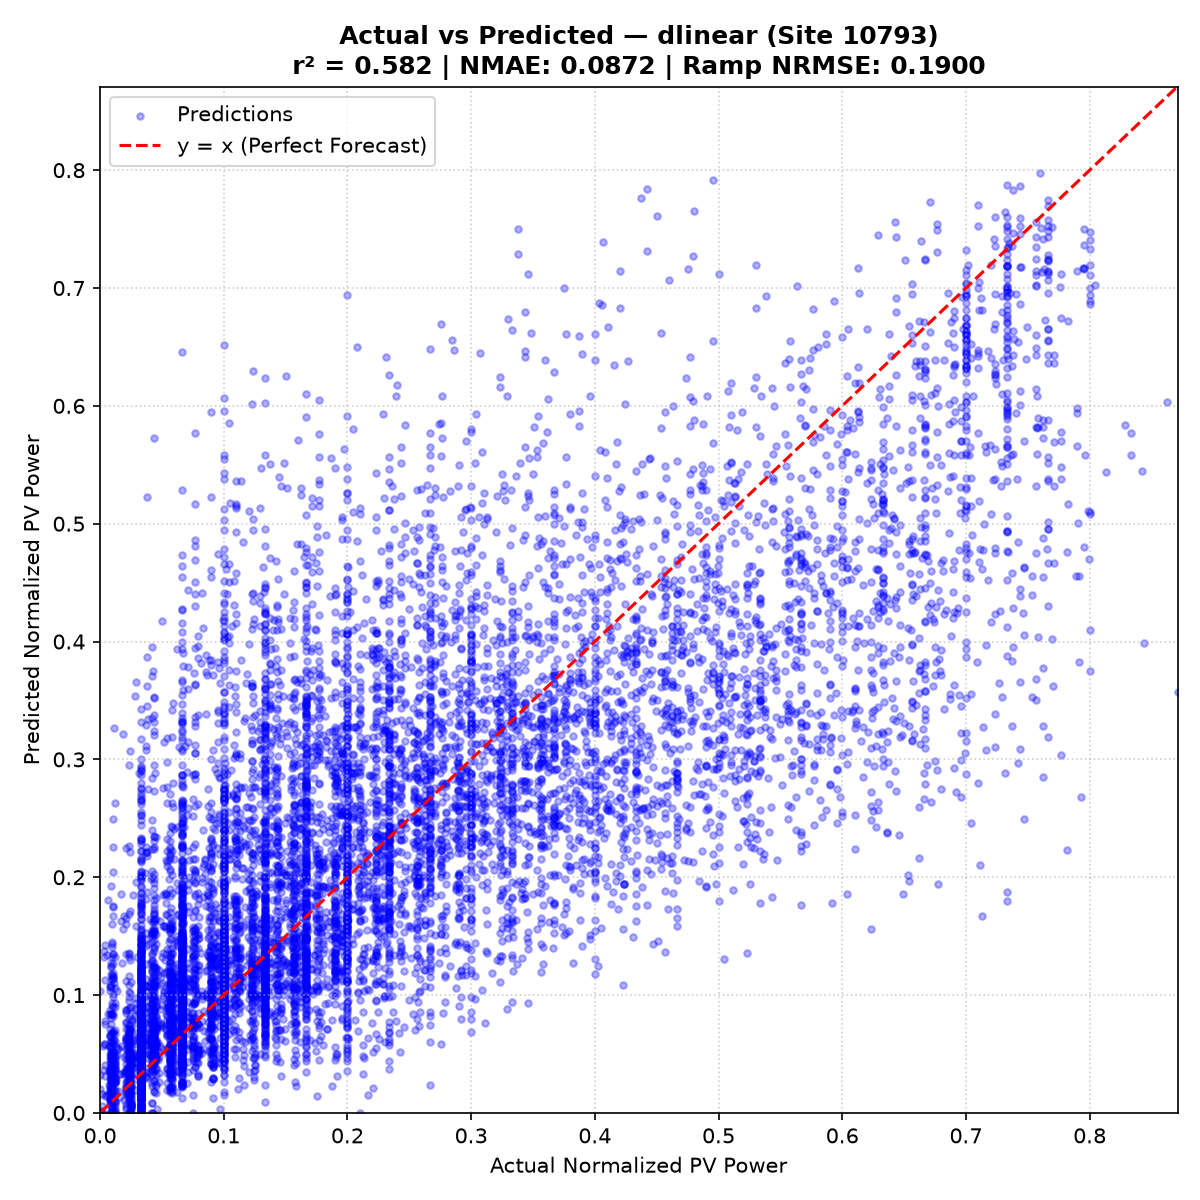
\includegraphics[width=\textwidth]{figures/scatter_dlinear.png}
\end{minipage}

\vspace{0.35cm}

\begin{minipage}{0.48\textwidth}
  \centering
  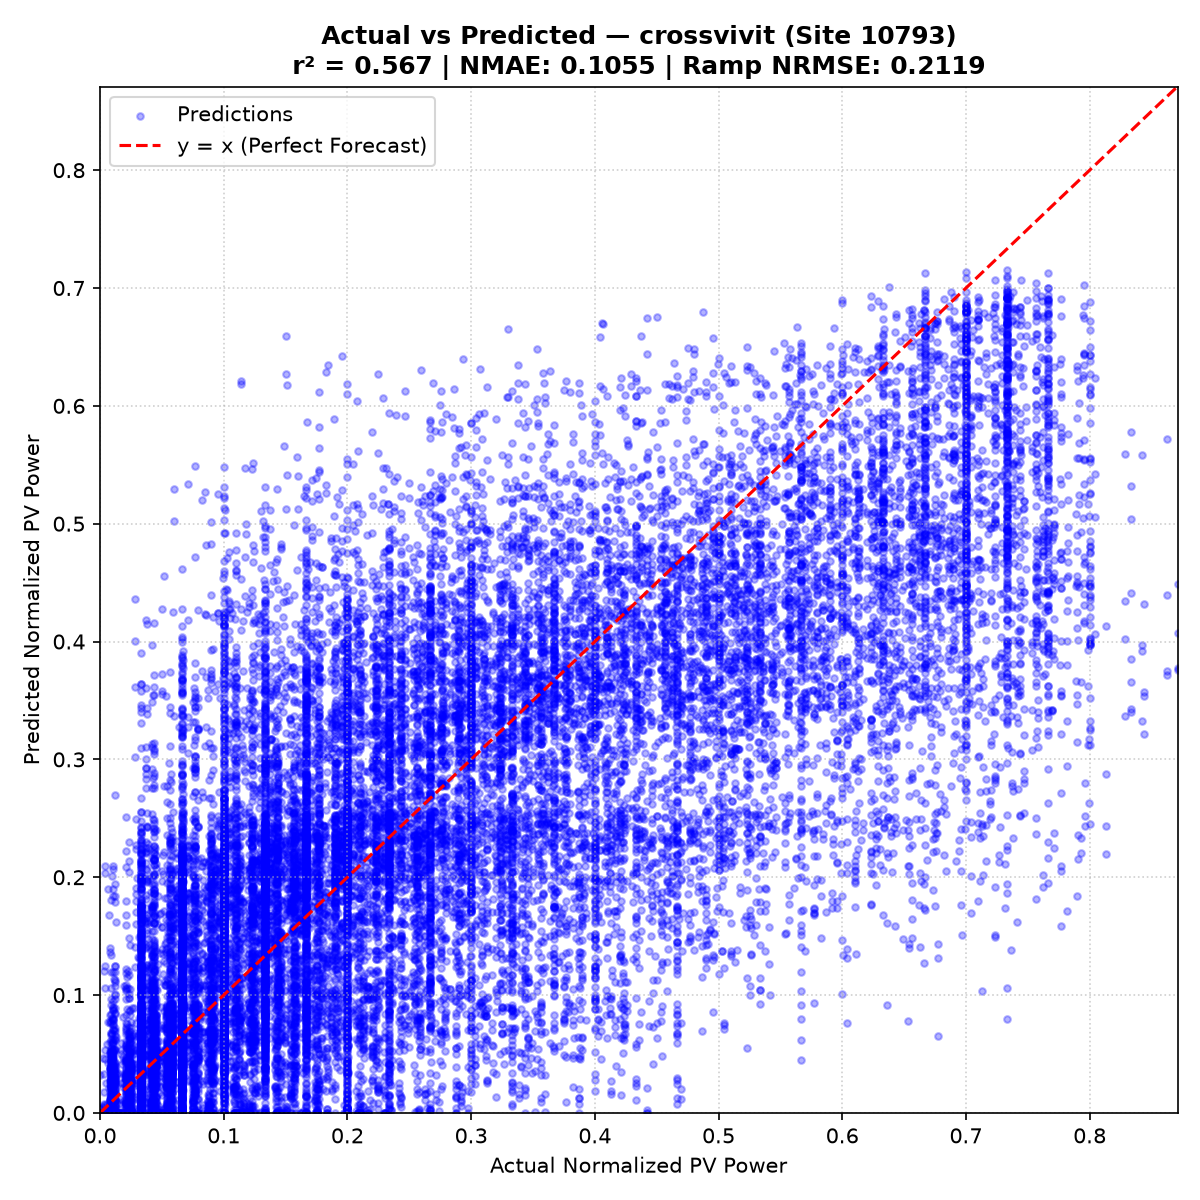
\includegraphics[width=\textwidth]{figures/scatter_crossvivit.png}
\end{minipage}
\hfill
\begin{minipage}{0.48\textwidth}
  \centering
  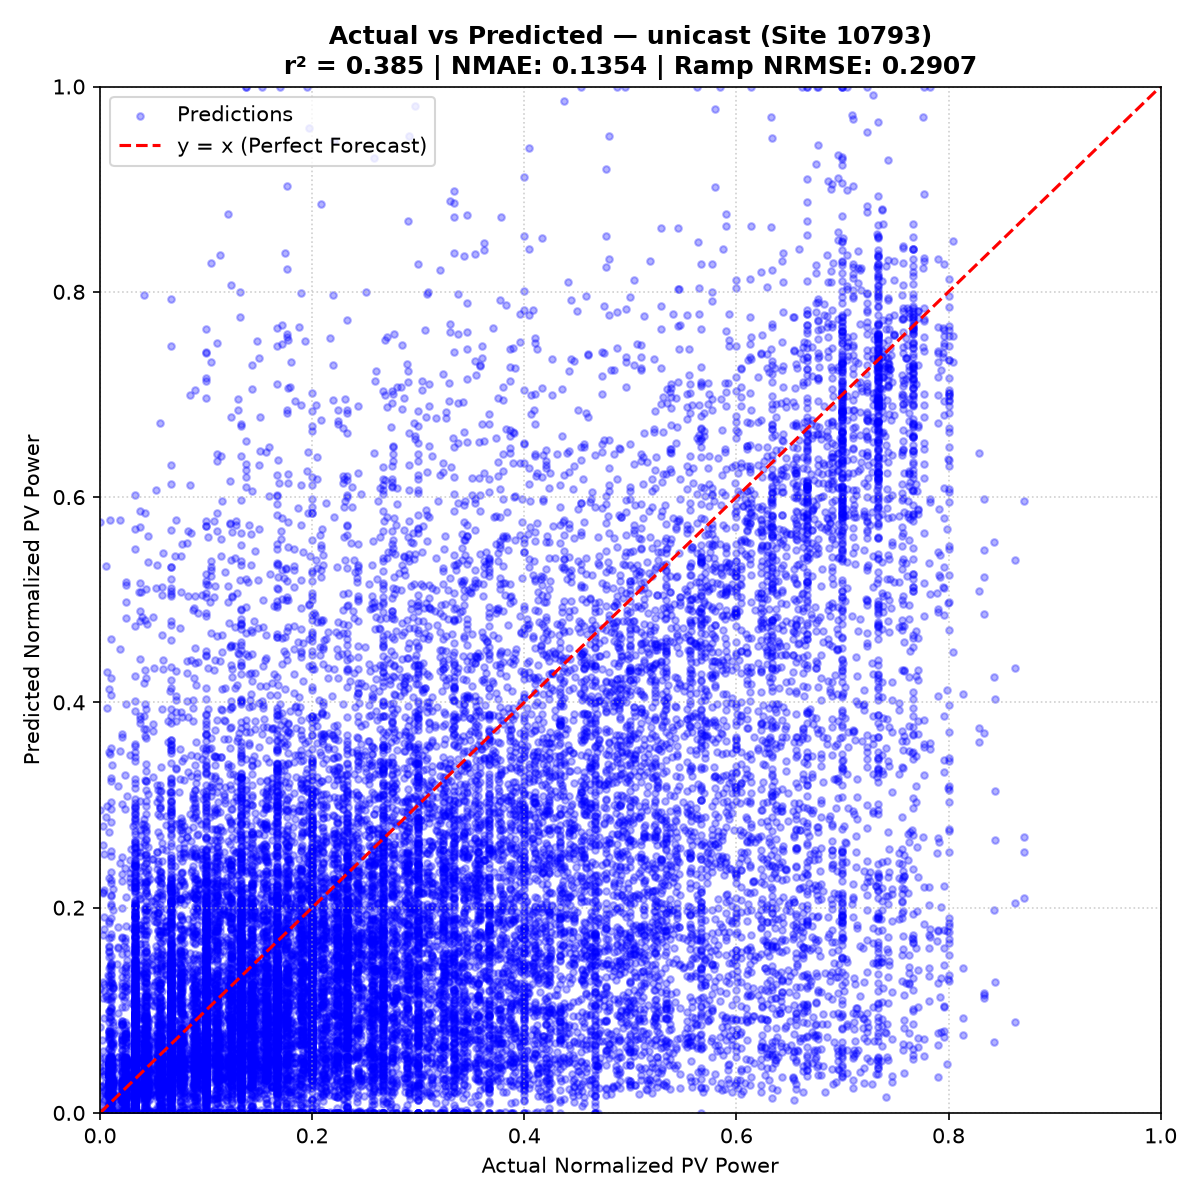
\includegraphics[width=\textwidth]{figures/scatter_unicast.png}
\end{minipage}
\caption{Calibration across tiers, same test site. Top: LightGBM and DLinear, the classical
and linear references --- both well centred, DLinear visibly more dispersed. Bottom:
CrossViVit and UniCast, two exogenous multimodal models, both showing the compression toward
the mean that produces high $R^2$ with low skill.}
\label{fig:scatter-tiers}
\end{figure}

\begin{figure}[h!]
\centering
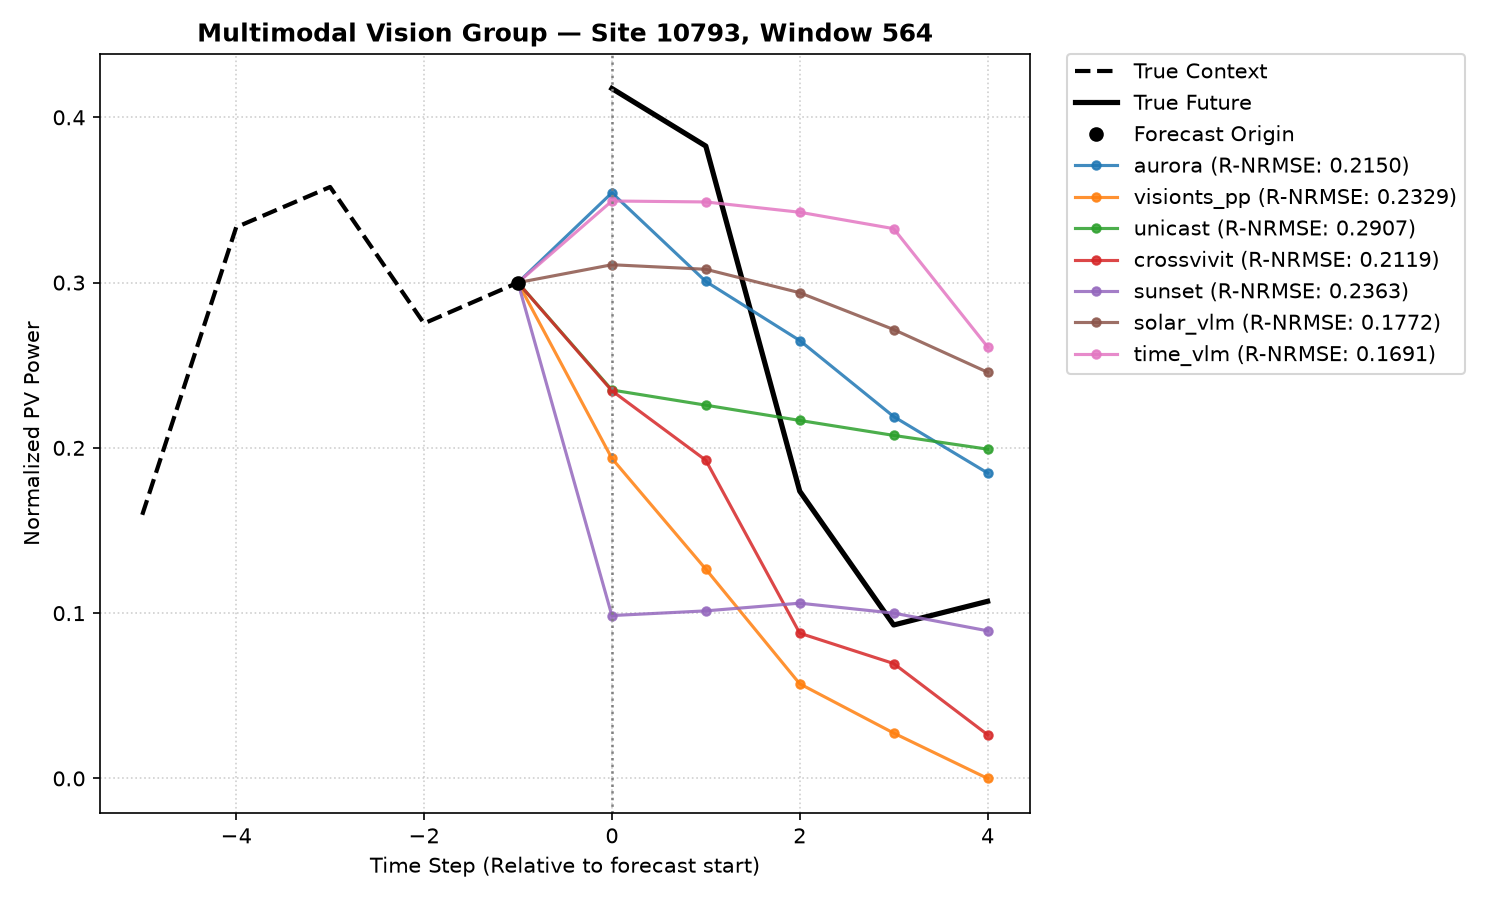
\includegraphics[width=0.92\textwidth]{figures/traces_multimodal.png}
\caption{The multimodal tier alone, same window as Figure~\ref{fig:traces}. The seven models
disagree by more than the whole range of the truth. Time-VLM and Solar-VLM hold output high;
SUNSET collapses immediately to 0.10 and stays there; VisionTS++ and CrossViVit decay to near
zero. All of them consume --- or in Time-VLM's case simulate --- a visual modality, and no two
of them read this window the same way.}
\label{fig:traces-mm}
\end{figure}

Figure~\ref{fig:traces-mm} is worth more attention than its aggregate row. The spread among
multimodal models on a single window exceeds the spread of the entire leaderboard: at the
final horizon step, predictions range from 0.00 (VisionTS++) to 0.26 (Time-VLM) against a
truth of 0.11. Two models overshoot by more than a factor of two, two undershoot to nothing,
and one --- SUNSET --- ignores the horizon entirely and outputs a near-constant. A visual
modality is evidently not a stabilising influence; it is a source of variance that each
architecture converts differently, which is consistent with the interface-loss explanation of
Section~\ref{sec:finding4}.

\section{The ramp regime}
\label{sec:ramp-results}

Appendix~\ref{app:ramp} reports every model on the top-decile $|\Delta y|$ subset. Three
observations follow, and they matter more for the thesis than the aggregate table does,
because the ramp regime is where the multimodal hypothesis was supposed to pay.

First, the ordering is broadly preserved but compressed. Time-VLM leads at 0.172 ramp NRMSE,
iTransformer follows at 0.177, and the reference floor sits at 0.281 --- a range of 0.109
against a range of 0.147 in the aggregate NRMSE column. Ramps are hard for everyone, and the
spread between a good model and a bad one narrows exactly where the value of forecasting is
highest.

Second, the retrieval models lose their advantage. TS-RAG and Cross-RAG rank fourth and fifth
overall but seventh and eighth on ramp NRMSE, behind Solar-VLM and PatchTST. This supports the
reading of Section~\ref{sec:finding3}: retrieval supplies level calibration and typical-case
accuracy more than it supplies transition dynamics. Retrieving a window that looks like the
current one is most useful when the current one is unremarkable.

Third --- and this is the observation that shapes Chapter~\ref{cha:expdesign} --- the model
with the best ramp accuracy in the entire suite consumes no external imagery. If satellite
frames were being exploited for advection, the exogenous tier should own this column. It does
not: Solar-VLM is fourth, CrossViVit sixteenth, SUNSET nineteenth. Whatever the cloud-state
information demonstrated in Figure~\ref{fig:cloud-residual} is worth, no current architecture
in this suite is extracting it in the regime where it should matter most.

\section{Practical considerations}
\label{sec:practical}

Accuracy is not the only axis on which these models differ, and a benchmark that ignores cost
gives misleading guidance to anyone who has to deploy something.

\paragraph{Cost of adaptation.} The three adaptation strategies differ by orders of magnitude
in what they require. Retrieval needs an index over training-plant windows and a
nearest-neighbour lookup at inference; no gradients, no accelerator, and a new plant can be
served the moment its history arrives. Adapter tuning needs a short training run over a small
parameter set. Full fine-tuning needs a training run over the whole backbone and produces a
task-specific copy of a large model that must then be stored and served. That the cheapest of
the three is also the most accurate on this task (Section~\ref{sec:finding3}) is the most
practically consequential finding in the chapter.

\paragraph{Cost of the visual branch.} Every exogenous multimodal model in the suite requires
a satellite ingest pipeline: reprojection, per-site cropping, storage of terabytes of frames,
and a vision encoder forward pass per forecast. In this study that pipeline is the single
largest engineering component of the dataset (Section~\ref{sec:sources}) and the vision
encoder dominates inference cost. The endogenous alternative --- rendering the series as an
image --- requires none of it. Against that background, Time-VLM outranking every
satellite-consuming model is not merely a scientific result but an economic one.

\paragraph{Serving a growing fleet.} The deployment scenario that motivated this thesis ---
new plants arriving continuously --- favours methods whose marginal cost per plant is near
zero. Supervised in-domain models, including the leader, must be retrained as the fleet
grows if they are to exploit new plants; zero-shot and retrieval methods absorb a new plant
by adding rows to an index. The leaderboard ordering and the operational ordering are
therefore not the same, and a practitioner reading only Table~\ref{tab:leaderboard} would
draw the wrong conclusion.

\section{What the benchmark cannot answer}
\label{sec:benchmark-limits}

Four questions are outside what these numbers support, and stating them prevents
over-reading.

\paragraph{Whether the results transfer to another fleet.} Everything here is
\texttt{uk\_pv}: one country, one satellite product, one capacity class, two years. The
\texttt{goes\_pvdaq} track exists in the dataset and differs in sensor, scale, latitude and
cadence, but was not run. Cross-dataset generalisation is unproven --- not disproven.

\paragraph{Whether the ordering is statistically significant.} Each model was run once, and
no significance testing accompanies the table. Differences of a few thousandths of skill ---
TS-RAG at 0.478 against Cross-RAG at 0.477, for instance --- are ties, and are read as such
throughout.

\paragraph{Whether the models were equally well tuned.} Hyperparameter budgets were
comparable but not identical, and vendored implementations carry their authors' defaults.
A model can lose a benchmark because its architecture is unsuited or because nobody tuned it,
and this study cannot fully separate the two. The tier structure mitigates rather than
eliminates the concern: within Tier~2, four models share one trainer, so differences there are
architectural.

\paragraph{Whether the models would rank the same at another horizon.} Every number here is a
six-hour forecast. At one hour persistence-like methods are far stronger and the spread
compresses; at twenty-four hours the observed cloud field is irrelevant and numerical weather
dominates, which would penalise every imagery-consuming model and favour those that ingest
the covariate track well. The skill-decay scenario that would settle this was only partially
run, so the ordering reported should be read as an ordering \emph{at six hours}.

\paragraph{Whether better conditioning would change the ordering.} The oracle rows show that
the same backbone gains 0.173 skill from privileged future weather. It is entirely possible
that the ranking of architectures would reorder under better --- but still legitimate ---
conditioning, and nothing here rules that out.

\section{What the benchmark establishes}
\label{sec:bar}

Three numbers define the target for any proposed architecture on this task.

\begin{itemize}
  \item \textbf{0.552} --- the overall bar (iTransformer). A model that does not approach it
    has not beaten supervised in-domain training.
  \item \textbf{0.540} --- the multimodal bar (Time-VLM), achieved with no external imagery.
  \item \textbf{0.331} --- the honest same-backbone reference (Chronos-2 fine-tuned). Any
    architecture built on Chronos-2 must clear this to show that its additions, rather than
    its backbone, are doing the work.
\end{itemize}

A fourth number is not a bar but a measurement of available headroom. The oracle variants,
which see observed future weather, reach 0.474 and 0.504 against 0.331 for the honest
fine-tuned model --- a gap of \textbf{0.173 skill} attributable purely to better conditioning
over the horizon. That is larger than the difference between any two architectures in the
entire suite. It is the single strongest indication in this work of where effort should be
directed, and Chapter~\ref{cha:conclusion} returns to it.

\par

